\begin{answer}
	\begin{figure}[H]
		\centering
		\vspace{-2mm}
		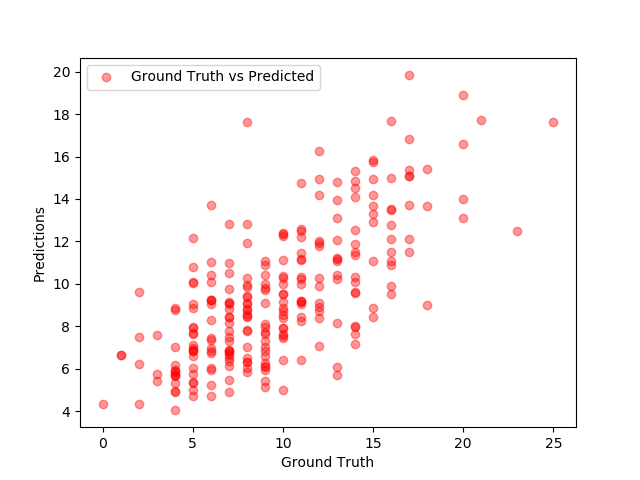
\includegraphics[width=0.65\linewidth]{../src/poisson/poisson_valid.png}
		\caption{Ground Truth vs Prediction plot on the validation set}
	\end{figure}


Note: Depending on the initial value of $\theta$, the final value of $\theta$ may be different. However, the log-likelihoods and predictions are nearly identical. This happens because of the way the data was simulated. $x_1$ is set to 0 or 1, and $x_2 = 1 - x_1$. Then, with the intercept term, $\theta_0 + \theta_1 x_1 + \theta_2 (1-x_1) = (\theta_0 + \theta_2) + (\theta_1 - \theta_2) x_1$. So we can only recover $(\theta_0 + \theta_2)$, $(\theta_1 - \theta_2)$, $\theta_3$, and $\theta_4$.

\end{answer}
